% =====================================================================
%  TEMPLATE BEAMER — SOUTENANCE DE MÉMOIRE  (UM · Free Mobile · Beemo)
%  Design : ivoire sobre + accent corail (Université de Montpellier),
%           serif (titres) / sans (corps), bandeau partenaires sur cartouches blancs.
%  Moteur : XeLaTeX ou LuaLaTeX  (compiler avec --shell-escape PAS requis)
%  Compilation :  xelatex soutenance.tex   (x2 pour les refs/remember picture)
%             ou  latexmk -xelatex soutenance.tex
%
%  Polices (chargées par NOM DE FICHIER .otf : présentes dans TeX Live,
%  aucune installation système requise) :
%    - Source Serif 4   (titres)   — paquet TeX Live « sourceserif »
%    - Source Sans 3    (corps)    — paquet TeX Live « sourcesans »
%    - JetBrains Mono   (code)     — paquet TeX Live « jetbrainsmono-otf »
%  Pour utiliser des polices installées sur le système, remplacez le bloc
%  « POLICES » par \setsansfont{Source Sans 3} / \setmonofont{JetBrains Mono},
%  etc. En dernier recours, Latin Modern Roman / Latin Modern Sans (toujours
%  disponibles) font l'affaire.
%
%  LOGOS : fichiers dans  assets/logo-um.png , assets/logo-free.png ,
%  assets/logo-beemo.png  (les fonds blancs Free/Beemo se fondent dans les
%  cartouches blancs \logochip). Ajustez les hauteurs au besoin.
% =====================================================================

\documentclass[aspectratio=169,11pt,t]{beamer}

% ---------- Dimensions du canevas ------------------------------------
% Le design est conçu sur un grand canevas 16:9. On agrandit la page
% (en conservant le ratio) : tailles de police et graphismes absolus se
% « dézooment » alors proportionnellement, le tout respire et rien n'est
% coupé. Les projecteurs/visionneuses ajustent à l'écran (seul le ratio
% compte). Pour revenir au format compact, supprimer cette ligne.
\geometry{paperwidth=240mm,paperheight=135mm}

% ---------- Polices (fontspec : nécessite XeLaTeX/LuaLaTeX) ----------
% Chargement par nom de fichier .otf : kpathsea/luaotfload trouve les
% fichiers dans l'arborescence TeX Live sans passer par fontconfig.
\usepackage{fontspec}
\setsansfont{SourceSans3}[
  Extension   = .otf,
  UprightFont = *-Regular,
  BoldFont    = *-Semibold,
  ItalicFont  = *-RegularIt,
  BoldItalicFont = *-SemiboldIt ]
\newfontfamily\seriffont{SourceSerif4}[
  Extension   = .otf,
  UprightFont = *-Regular,
  BoldFont    = *-Semibold,
  ItalicFont  = *-RegularIt,
  BoldItalicFont = *-SemiboldIt ]
\setmonofont{JetBrainsMono}[
  Extension   = .otf,
  UprightFont = *-Regular,
  BoldFont    = *-SemiBold,
  ItalicFont  = *-Italic,
  BoldItalicFont = *-SemiBoldItalic,
  Scale       = 0.86 ]
\renewcommand{\familydefault}{\sfdefault}   % corps en sans par défaut

% ---------- Langue ----------
\usepackage{polyglossia}
\setdefaultlanguage{french}

% ---------- Paquets graphiques ----------
\usepackage{tikz}
\usetikzlibrary{arrows.meta,positioning,calc}
\usepackage{booktabs}
\usepackage{colortbl}
\usepackage{listings}
\usepackage{graphicx}

% --- Logo partenaire sur cartouche blanc à hauteur FIXE (logos harmonisés) ---
% \logochip{fichier}{hauteur-logo}{hauteur-cartouche} : logo centré verticalement.
% La hauteur de cartouche est commune à une rangée ; la hauteur de logo est
% ajustée par image pour égaliser le poids optique (sceau carré = un peu plus petit).
\newcommand{\logochip}[3]{%
  \colorbox{white}{%
    \raisebox{-0.5\height}{\rule{0pt}{#3}}\kern2pt%
    \raisebox{-0.5\height}{\includegraphics[height=#2]{assets/#1}}\kern2pt}}

% --- Cartouche logo BORDÉ (comme les cartouches blancs de la page de titre HTML :
%     fond blanc, fin liseré ivoire). Mêmes arguments que \logochip. ---
\newcommand{\logocard}[3]{%
  \fcolorbox{chiprule}{white}{%
    \raisebox{-0.5\height}{\rule{0pt}{#3}}\kern2pt%
    \raisebox{-0.5\height}{\includegraphics[height=#2]{assets/#1}}\kern2pt}}

% =====================================================================
%  PALETTE
% =====================================================================
\definecolor{accent}{HTML}{D8524A}   % corail Université de Montpellier
\definecolor{accentlt}{HTML}{F7CFC9} % corail clair (sur fond foncé)
\definecolor{freeRed}{HTML}{E2001A}  % rouge Free Mobile
\definecolor{beemoBlue}{HTML}{1B8ED4}% bleu Beemo
\definecolor{dark}{HTML}{1B1A17}     % fond sombre des séparateurs de section
\definecolor{bg}{HTML}{F6F4EF}       % ivoire (fond des slides)
\definecolor{sectionbg}{HTML}{ECE3D6}% sable chaud (fond des transitions de section)
\definecolor{panel}{HTML}{ECEAE3}    % panneau teinté
\definecolor{ink}{HTML}{1C1B18}      % presque noir
\definecolor{ink2}{HTML}{3A382F}     % gris foncé (corps secondaire)
\definecolor{stone}{HTML}{56524A}    % gris chaud (sous-titre, légendes, citation)
\definecolor{muted}{HTML}{7A766C}    % gris légende / pied de page
\definecolor{rule}{HTML}{DDD8CF}     % filets fins
\definecolor{chiprule}{HTML}{E4DFD6} % bordure des cartouches logos (page de titre)
\definecolor{codebg}{HTML}{24302F}   % fond bloc de code
\definecolor{codehead}{HTML}{1C2625} % barre de titre du bloc de code (chrome)
\definecolor{codefg}{HTML}{DFE7E3}   % texte code
\definecolor{codekw}{HTML}{7FA8B5}   % mots-clés
\definecolor{codefn}{HTML}{E7C97F}   % fonctions
\definecolor{codenum}{HTML}{C69A6B}  % nombres
\definecolor{codecmt}{HTML}{6F7E7A}  % commentaires
\definecolor{codedim}{HTML}{8A948F}  % nom de fichier (chrome)
\definecolor{dotred}{HTML}{E06C5A}   % pastille « feu » rouge
\definecolor{dotyellow}{HTML}{E0B54A}% pastille « feu » jaune
\definecolor{dotgreen}{HTML}{5AA86F} % pastille « feu » verte

% =====================================================================
%  THÈME — réglages globaux
% =====================================================================
\setbeamercolor{background canvas}{bg=bg}
\setbeamercolor{normal text}{fg=ink}
\setbeamercolor{itemize item}{fg=accent}
\setbeamercolor{itemize subitem}{fg=accent}
\usebeamercolor[fg]{normal text}

\setbeamertemplate{navigation symbols}{}      % pas de barre de navigation
\setbeamersize{text margin left=1.1cm,text margin right=1.1cm}

% ----- Puces carrées accent -----
\setbeamertemplate{itemize item}{\raisebox{0.18ex}{\textcolor{accent}{\rule{1.6ex}{1.6ex}}}}
\setbeamertemplate{itemize subitem}{\textcolor{accent}{\textbf{--}}}

% ----- Titre de frame : serif, accent, filet dessous -----
\setbeamertemplate{frametitle}{%
  \vspace*{0.55cm}%
  {\seriffont\bfseries\color{accent}\fontsize{20}{24}\selectfont\insertframetitle\par}%
  \vspace*{0.18cm}%
  {\color{accent}\rule{1.55cm}{2.2pt}}\par
  \vspace*{0.30cm}%
}

% ----- Pied de page : nom | logos partenaires | carré accent + n° -----
\setbeamertemplate{footline}{%
  % filet de séparation (cf. border-top du rendu HTML)
  \hbox to\paperwidth{\hskip1.1cm{\color{rule}\rule{\dimexpr\paperwidth-2.2cm\relax}{0.4pt}}\hskip1.1cm}%
  \vskip2.5pt%
  \hbox{%
    \begin{beamercolorbox}[wd=\paperwidth,ht=3.0ex,dp=2.2ex,leftskip=1.1cm,rightskip=1.1cm]{}%
      \usebeamerfont{normal text}\fontsize{7}{9}\selectfont\color{muted}%
      \insertshortauthor\ — \insertshorttitle\hfill
      {\setlength{\fboxsep}{1.5pt}%
       \logochip{logo-um.png}{0.30cm}{0.34cm}\hspace{3pt}%
       \logochip{logo-free.png}{0.27cm}{0.34cm}\hspace{3pt}%
       \logochip{logo-beemo.png}{0.21cm}{0.34cm}}\hspace{10pt}%
      \textcolor{accent}{\rule{0.9ex}{0.9ex}}\ \insertframenumber%
    \end{beamercolorbox}}%
  \vskip2pt%
}

% =====================================================================
%  COMMANDES UTILITAIRES
% =====================================================================
% --- Diapositive de séparation de section (fond sombre + graphisme tri-marques) -
% Usage : \sectionslide{01}{Titre de section}{Phrase de transition.}
% Composition : cercles aux couleurs UM / Free / Beemo (mode « screen »),
% barre tricolore, légende de rappel des couleurs en bas de page.
\newcommand{\sectionslide}[3]{%
\begingroup
\setbeamercolor{background canvas}{bg=sectionbg}
\begin{frame}[plain,t]
  % --- composition graphique (nécessite 2 compilations pour remember picture) ---
  \begin{tikzpicture}[remember picture,overlay]
    \coordinate (cl) at ($(current page.north east)+(-2.55,-3.75)$);
    % anneaux décoratifs (rappel d'orbite / mouvement)
    \draw[ink!16!sectionbg,line width=1pt,dash pattern=on 3pt off 5pt] (cl) circle (3.05);
    \draw[ink!10!sectionbg,line width=0.6pt] (cl) circle (2.15);
    % cercles des 3 marques (mode « multiply » pour un fond clair)
    \begin{scope}[blend mode=multiply]
      \fill[accent,opacity=0.55]    ($(cl)+(-0.5,1.05)$)  circle (2.35);
      \fill[freeRed,opacity=0.55]   ($(cl)+(1.1,-0.15)$)  circle (2.35);
      \fill[beemoBlue,opacity=0.55] ($(cl)+(-0.5,-0.85)$) circle (2.35);
    \end{scope}
    % satellites sur les orbites
    \fill[accent]    ($(cl)+(62:3.05)$)  circle (0.15);
    \fill[beemoBlue] ($(cl)+(232:2.15)$) circle (0.11);
  \end{tikzpicture}
  % --- contenu ---
  \vspace*{2.0cm}
  {\seriffont\bfseries\fontsize{84}{84}\selectfont\textcolor{accent!24!sectionbg}{#1}\par}
  \vspace*{0.20cm}
  \hbox{\textcolor{accent}{\rule{0.7cm}{2.6pt}}\textcolor{freeRed}{\rule{0.7cm}{2.6pt}}%
    \textcolor{beemoBlue}{\rule{0.7cm}{2.6pt}}\hspace{0.32cm}%
    \raisebox{0.06cm}{\bfseries\fontsize{11}{11}\selectfont\textcolor{stone}{\MakeUppercase{Partie}~#1}}}\par
  \vspace*{0.30cm}
  {\seriffont\bfseries\fontsize{30}{34}\selectfont\textcolor{ink}{#2}\par}
  \vspace*{0.24cm}
  {\fontsize{12}{16}\selectfont\textcolor{stone}{#3}\par}
  \vfill
  % --- rappel des couleurs des entreprises ---
  \hbox{%
    \raisebox{0.12ex}{\textcolor{accent}{\rule{1.4ex}{1.4ex}}}\ {\fontsize{9}{11}\selectfont\textcolor{stone}{Université de Montpellier}}\hspace{0.7cm}%
    \raisebox{0.12ex}{\textcolor{freeRed}{\rule{1.4ex}{1.4ex}}}\ {\fontsize{9}{11}\selectfont\textcolor{stone}{Free Mobile}}\hspace{0.7cm}%
    \raisebox{0.12ex}{\textcolor{beemoBlue}{\rule{1.4ex}{1.4ex}}}\ {\fontsize{9}{11}\selectfont\textcolor{stone}{Beemo Technologie}}}
  \vspace*{0.7cm}
\end{frame}
\endgroup}

% --- « Gros chiffre » clé --------------------------------------------
\newcommand{\bignum}[2]{%
  {\seriffont\bfseries\fontsize{46}{46}\selectfont\textcolor{accent}{#1}}\\[2pt]
  {\fontsize{11}{14}\selectfont\textcolor{stone}{#2}}}

% =====================================================================
%  COMPOSANTS GRAPHIQUES — cartes & flux (pour « dégraisser » le texte)
% =====================================================================
% --- Carte : marqueur accent + titre serif + corps, fond blanc bordé,
%     hauteur fixe pour égaliser les rangées. \card{hauteur}{titre}{corps} ---
\newcommand{\card}[3]{%
  \setlength{\fboxsep}{11pt}%
  \fcolorbox{rule}{white}{%
    \begin{minipage}[t][#1][t]{\dimexpr\linewidth-24pt\relax}
      {\seriffont\bfseries\fontsize{13}{16}\selectfont\color{ink}%
        \raisebox{0.18ex}{\textcolor{accent}{\rule{1.2ex}{1.2ex}}}\ #2\par}
      \vspace{4.5pt}
      {\fontsize{10}{13.5}\selectfont\color{ink2}#3\par}
    \end{minipage}}}

% --- Carte « sombre » (accent plein) pour un point fort / une chute ---
\newcommand{\cardhi}[3]{%
  \setlength{\fboxsep}{11pt}%
  \colorbox{accent}{%
    \begin{minipage}[t][#1][t]{\dimexpr\linewidth-24pt\relax}
      {\seriffont\bfseries\fontsize{13}{16}\selectfont\color{bg}%
        \raisebox{0.18ex}{\textcolor{bg}{\rule{1.2ex}{1.2ex}}}\ #2\par}
      \vspace{4.5pt}
      {\fontsize{10}{13.5}\selectfont\color{bg!92}#3\par}
    \end{minipage}}}

% --- Styles TikZ pour diagrammes de flux ----------------------------
\tikzset{
  flowbox/.style={draw=accent,line width=1.2pt,fill=white,rounded corners=6pt,
                  minimum height=1.9cm,text width=4.0cm,align=center,
                  font=\sffamily,inner sep=8pt},
  flowhi/.style={fill=accent,rounded corners=6pt,
                 minimum height=1.9cm,text width=4.0cm,align=center,
                 font=\sffamily,text=bg,inner sep=8pt},
  flowarr/.style={-{Stealth[length=4mm,width=4mm]},accent,line width=1.8pt},
}
% Contenu d'un nœud de flux : titre gras + détail gris.
\newcommand{\flowtxt}[2]{{\bfseries\fontsize{12}{14}\selectfont #1}\\[2pt]{\fontsize{9}{11.5}\selectfont\color{ink2}#2}}
\newcommand{\flowtxthi}[2]{{\bfseries\fontsize{12}{14}\selectfont #1}\\[2pt]{\fontsize{9}{11.5}\selectfont\color{bg!88}#2}}

% --- Style des blocs de code (listings) ------------------------------
\lstdefinestyle{soutenance}{
  backgroundcolor=\color{codebg},
  basicstyle=\ttfamily\fontsize{10}{13}\selectfont\color{codefg},
  keywordstyle=\color{codekw}\bfseries,
  emphstyle=\color{codefn},
  commentstyle=\color{codecmt}\itshape,
  numberstyle=\tiny\color{codecmt},
  stringstyle=\color{accentlt},
  showstringspaces=false,
  breaklines=true,
  tabsize=4,
  xleftmargin=16pt,xrightmargin=0pt,
  framexleftmargin=16pt,framexrightmargin=0pt,
  aboveskip=0pt,belowskip=0pt,
  frame=none,
  language=Python,
  emph={descente_gradient,gradient,range}
}

% --- Barre de titre « fenêtre » du bloc de code (3 pastilles + nom de fichier),
%     reprenant le chrome du rendu HTML. À placer JUSTE au-dessus du lstlisting
%     (suivie de \par\nointerlineskip) ; sa largeur épouse celle de la colonne,
%     comme le fond du listing (xleftmargin/framexleftmargin = 16pt, droite à 0). ---
\newcommand{\codetitlebar}[1]{%
  {\setlength{\fboxsep}{0pt}%
   \colorbox{codehead}{\makebox[\linewidth][l]{%
     \rule[-0.95ex]{0pt}{3.0ex}%
     \hspace{14pt}%
     \tikz{\fill[dotred]    (0,0) circle (2.2pt);}\hspace{4.5pt}%
     \tikz{\fill[dotyellow] (0,0) circle (2.2pt);}\hspace{4.5pt}%
     \tikz{\fill[dotgreen]  (0,0) circle (2.2pt);}\hspace{13pt}%
     {\ttfamily\fontsize{8.5}{10}\selectfont\color{codedim}#1}\hfill}}}}

% =====================================================================
%  MÉTADONNÉES  — adaptées au mémoire (à ajuster si besoin)
% =====================================================================
\title{Réduction de la dette technique dans un environnement de production}
\author{Jérémy Hurel}
\institute{Université de Montpellier · Faculté des Sciences}
\date{2026}

% versions courtes pour le pied de page
\newcommand{\shortname}{Jérémy Hurel}
\newcommand{\shortwork}{Soutenance de mémoire}

\begin{document}

% =====================================================================
%  DIAPOSITIVES — une diapo par fichier dans slides/
% =====================================================================
% =====================================================================
%  1 — PAGE DE TITRE
% =====================================================================
\begin{frame}[plain]
  \vspace*{1.6cm}
  {\bfseries\fontsize{9}{9}\selectfont\textcolor{accent}{\MakeUppercase{Soutenance de mémoire de fin d'études}}\par}
  \vspace*{0.30cm}
  {\color{accent}\rule{1.8cm}{2.6pt}}\par
  \vspace*{0.45cm}
  {\seriffont\bfseries\fontsize{27}{31}\selectfont\textcolor{ink}%
    {Réduction de la dette technique\\ dans un environnement de production}\par}
  \vspace*{0.28cm}
  {\seriffont\itshape\fontsize{14}{18}\selectfont\textcolor{stone}%
    {Master 2 Informatique — parcours Génie Logiciel · deux années d'alternance}\par}
  \vspace*{0.85cm}
  % --- bloc auteur / encadrement ---
  \begin{columns}[t]
    \column{0.30\textwidth}
      {\fontsize{7.5}{9}\selectfont\textcolor{muted}{\MakeUppercase{Présenté par}}\par}
      \vspace{2pt}{\bfseries\fontsize{11}{13}\selectfont\textcolor{ink}{Jérémy Hurel}}
    \column{0.38\textwidth}
      {\fontsize{7.5}{9}\selectfont\textcolor{muted}{\MakeUppercase{Tuteur universitaire}}\par}
      \vspace{2pt}{\fontsize{11}{13}\selectfont\textcolor{ink2}{Mickaël Montassier — Univ.\ de Montpellier}}
    \column{0.30\textwidth}
      {\fontsize{7.5}{9}\selectfont\textcolor{muted}{\MakeUppercase{Tuteur entreprise}}\par}
      \vspace{2pt}{\fontsize{11}{13}\selectfont\textcolor{ink2}{David Desmarest — Free · Beemo}}
  \end{columns}
  \vspace{0.85cm}
  % --- bandeau partenaires ---
  {\fontsize{7.5}{9}\selectfont\textcolor{muted}{\MakeUppercase{Mémoire réalisé chez}}\par}
  \vspace{0.24cm}
  \makebox[\linewidth][l]{{\setlength{\fboxsep}{5pt}%
    \logocard{logo-um.png}{0.95cm}{1.05cm}\hspace{6pt}%
    \logocard{logo-free.png}{0.85cm}{1.05cm}\hspace{6pt}%
    \logocard{logo-beemo.png}{0.64cm}{1.05cm}}\hfill
    \raisebox{-0.5\height}{\fontsize{9}{11}\selectfont\textcolor{muted}{Année universitaire 2024 -- 2026}}}
\end{frame}

% =====================================================================
%  2 — FRISE CHRONOLOGIQUE DU PARCOURS
% =====================================================================
% Récit : arrivée chez Free Mobile (équipe Valo) → restructuration de
% l'équipe (incertitude, déclencheur du départ) → arrivée chez Beemo
% Technologie dans le sillage de David Desmarest → aujourd'hui.
% Code couleur : segment Free en rouge, segment Beemo en bleu, présent
% en corail (accent UM). Le dessin est mis à l'échelle de la largeur de
% texte (resizebox), comme le Gantt du mémoire.
\begin{frame}{Deux ans, deux entreprises}
  \vspace{0.45cm}
  \centering
  \resizebox{\textwidth}{!}{%
  \begin{tikzpicture}[font=\sffamily]
    % ----- ligne de temps : Free (rouge) jusqu'à l'arrivée Beemo, puis bleu -----
    \draw[freeRed,line width=3.2pt]   (1.0,0) -- (15.0,0);
    \draw[beemoBlue,line width=3.2pt] (15.0,0) -- (19.0,0);
    \draw[beemoBlue,line width=3.2pt,-{Stealth[length=4.5mm,width=4.5mm]}]
          (19.0,0) -- (20.1,0);

    % ----- marqueurs (halo ivoire pour détacher de la ligne) -----
    \foreach \x/\c in {1.5/freeRed, 6.0/freeRed, 10.5/freeRed, 15.0/beemoBlue, 19.0/accent}{
      \fill[bg]  (\x,0) circle (0.34);
      \fill[\c]  (\x,0) circle (0.21);
    }

    % ----- jalon 1 (haut) -----
    \draw[freeRed,line width=1pt] (1.5,0.34) -- (1.5,0.62);
    \node[anchor=south,align=center,text width=3.8cm] at (1.5,0.62){%
      {\bfseries\color{freeRed}\fontsize{11}{13}\selectfont Juillet 2024}\\[1.5pt]
      {\seriffont\bfseries\color{ink}\fontsize{13}{15}\selectfont Arrivée chez Free Mobile}\\[2pt]
      {\color{muted}\fontsize{9.5}{12}\selectfont Équipe Valo — Core SI}};

    % ----- jalon 2 (bas) ----- restructuration ~2-3 mois avant le départ de David (oct. 2025)
    \draw[freeRed,line width=1pt] (6.0,-0.34) -- (6.0,-0.62);
    \node[anchor=north,align=center,text width=3.8cm] at (6.0,-0.62){%
      {\bfseries\color{freeRed}\fontsize{11}{13}\selectfont Été 2025}\\[1.5pt]
      {\seriffont\bfseries\color{ink}\fontsize{13}{15}\selectfont Restructuration de l'équipe}\\[2pt]
      {\color{muted}\fontsize{9.5}{12}\selectfont Incertitude sur la conduite du développement à venir}};

    % ----- jalon 3 (haut) ----- démission posée en janv. 2026, préavis 2 mois
    \draw[freeRed,line width=1pt] (10.5,0.34) -- (10.5,0.62);
    \node[anchor=south,align=center,text width=3.8cm] at (10.5,0.62){%
      {\bfseries\color{freeRed}\fontsize{11}{13}\selectfont Janvier 2026}\\[1.5pt]
      {\seriffont\bfseries\color{ink}\fontsize{13}{15}\selectfont Démission de Free Mobile}\\[2pt]
      {\color{muted}\fontsize{9.5}{12}\selectfont Préavis de deux mois}};

    % ----- jalon 4 (bas) -----
    \draw[beemoBlue,line width=1pt] (15.0,-0.34) -- (15.0,-0.62);
    \node[anchor=north,align=center,text width=3.8cm] at (15.0,-0.62){%
      {\bfseries\color{beemoBlue}\fontsize{11}{13}\selectfont Avril 2026}\\[1.5pt]
      {\seriffont\bfseries\color{ink}\fontsize{13}{15}\selectfont Arrivée chez Beemo Technologie}\\[2pt]
      {\color{muted}\fontsize{9.5}{12}\selectfont Dans le sillage de David Desmarest}};

    % ----- jalon 5 (haut) -----
    \draw[accent,line width=1pt] (19.0,0.34) -- (19.0,0.62);
    \node[anchor=south,align=center,text width=3.4cm] at (19.0,0.62){%
      {\bfseries\color{accent}\fontsize{11}{13}\selectfont Aujourd'hui}\\[1.5pt]
      {\seriffont\bfseries\color{ink}\fontsize{13}{15}\selectfont Missions en cours}\\[2pt]
      {\color{muted}\fontsize{9.5}{12}\selectfont Juin 2026}};
  \end{tikzpicture}}
\end{frame}

% =====================================================================
%  3 — FIL ROUGE : la citation fondatrice de Ward Cunningham
% =====================================================================
\begingroup
\setbeamercolor{background canvas}{bg=panel}
\begin{frame}[plain,c]
  \begin{columns}\column{0.88\textwidth}
    {\seriffont\fontsize{60}{40}\selectfont\textcolor{accent}{“}\par}
    \vspace{0.1cm}
    {\seriffont\itshape\fontsize{22}{30}\selectfont\textcolor{ink}%
      {Livrer une première version du code, c'est comme s'endetter. Une petite
       dette accélère le développement à condition d'être remboursée rapidement
       par une réécriture.}\par}
    \vspace{0.6cm}
    \hbox{\textcolor{accent}{\rule{1.3cm}{2pt}}\hspace{0.35cm}%
      \raisebox{-0.35ex}{\fontsize{12}{14}\selectfont\textcolor{stone}%
        {Ward Cunningham, \textit{The WyCash Portfolio Management System}, 1992}}}
  \end{columns}
\end{frame}
\endgroup

% =====================================================================
%  5 — PLAN DE LA SOUTENANCE : les trois axes
% =====================================================================
% Deux parties : (1) les enjeux sociaux et de productivité qui motivent la
% réduction de la dette technique (dette technique, intérêt de l'IA, gains
% de productivité) ; (2) le cœur du propos, écrire du code de production
% dans une base déjà fortement endettée. Mise en page : gros numéros serif
% en accent, titres serif encre, descriptif en gris, filet de séparation.
\newcommand{\planitem}[3]{%
  \noindent
  \begin{minipage}[c]{1.85cm}%
    {\seriffont\bfseries\fontsize{38}{38}\selectfont\color{accent}#1}%
  \end{minipage}%
  \begin{minipage}[c]{\dimexpr\textwidth-1.95cm\relax}%
    {\seriffont\bfseries\fontsize{16}{20}\selectfont\color{ink}#2\par}%
    \vspace{2pt}%
    {\fontsize{10.5}{14}\selectfont\color{ink2}#3\par}%
  \end{minipage}\par}

\begin{frame}{Trois points qui me tiennent à cœur}
  \vspace{0.30cm}
  \planitem{01}{Les enjeux sociaux de la dette technique}%
    {Motivation des équipes, dette de connaissance et coût humain du legacy}

  \vspace{0.28cm}{\color{rule}\rule{\textwidth}{0.6pt}}\par\vspace{0.28cm}

  \planitem{02}{L'IA, une solution pleine de promesses}%
    {Un levier puissant mais conditionné, et ses propres risques de dette}

  \vspace{0.28cm}{\color{rule}\rule{\textwidth}{0.6pt}}\par\vspace{0.28cm}

  \planitem{03}{Écrire du code dans un existant fortement endetté}%
    {L'adressage incrémental et l'isolation du code neuf sur une base legacy}
\end{frame}

% =====================================================================
%  PARTIE 01 — LES ENJEUX SOCIAUX
% =====================================================================
\sectionslide{01}{Les enjeux sociaux de la dette technique}%
  {La forme de dette la plus dangereuse n'est pas dans le code : elle part avec les personnes.}

% =====================================================================
%  La dette n'est pas qu'un problème de code
% =====================================================================
\begin{frame}{La dette n'est pas qu'un problème de code}
  \vspace{0.30cm}
  \begin{columns}[t,onlytextwidth]
    \column{0.485\textwidth}
      \card{2.45cm}{Chronophage et ingrat}{Reprendre le contrôle d'un logiciel
        \emph{legacy} est un travail long, et peu gratifiant.}
    \column{0.485\textwidth}
      \card{2.45cm}{Un coût affectif mesuré}{La psychométrie l'observe : le code
        endetté génère déplaisir, anxiété, jusqu'à la réticence à intervenir.}
  \end{columns}
  \vspace{0.30cm}
  \begin{columns}[t,onlytextwidth]
    \column{0.485\textwidth}
      \card{2.45cm}{La « dette sociale »}{Des structures d'équipe sous-optimales
        génèrent, comme le code, un surcoût croissant.}
    \column{0.485\textwidth}
      \cardhi{2.45cm}{La motivation, un levier}{Pour résorber une dette, elle pèse
        autant que l'outillage ou l'architecture.}
  \end{columns}
\end{frame}

% =====================================================================
%  Deux engrenages : les deux spirales de la démotivation
% =====================================================================
\begin{frame}{Deux spirales, un même déclencheur}
  \vspace{0.55cm}
  \centering
  \resizebox{0.96\textwidth}{!}{%
  \begin{tikzpicture}[font=\sffamily,
      node distance=0.9cm,
      stp/.style={draw=accent,line width=1.3pt,fill=white,rounded corners=4pt,
                  minimum height=1.3cm,text width=3.4cm,align=center,
                  font=\bfseries\fontsize{11}{13}\selectfont,text=ink},
      bad/.style={fill=accent,rounded corners=4pt,minimum height=1.3cm,
                  text width=3.4cm,align=center,
                  font=\bfseries\fontsize{11}{13}\selectfont,text=bg},
      arr/.style={-{Stealth[length=4mm,width=4mm]},accent,line width=1.6pt}]
    \node[stp] (mot) {Perte de motivation};
    % spirale haute : départ -> perte de connaissance
    \node[stp,above right=0.4cm and 2.1cm of mot] (dem) {Démission};
    \node[bad,right=2.1cm of dem] (con) {Perte de connaissances};
    % spirale basse : ralentissement -> perte financière
    \node[stp,below right=0.4cm and 2.1cm of mot] (ral) {Ralentissement des livraisons};
    \node[bad,right=2.1cm of ral] (fin) {Perte financière};
    \draw[arr] (mot.east) to[out=30,in=180] (dem.west);
    \draw[arr] (dem) -- (con);
    \draw[arr] (mot.east) to[out=-30,in=180] (ral.west);
    \draw[arr] (ral) -- (fin);
  \end{tikzpicture}}
  \par\vspace{0.5cm}
  {\fontsize{10}{13}\selectfont\textcolor{muted}%
    {Un même déclencheur, la démotivation, alimente deux pertes : la connaissance et l'argent.}}
\end{frame}

% =====================================================================
%  Ce que j'ai observé chez Free Mobile
% =====================================================================
\begin{frame}{Ce que j'ai observé chez Free Mobile}
  \vspace{0.7cm}
  \centering
  \resizebox{\textwidth}{!}{%
  \begin{tikzpicture}[font=\sffamily,node distance=1.15cm]
    \node[flowbox] (a) {\flowtxt{Reprendre le contrôle}{du \emph{Valo Engine}, un logiciel critique}};
    \node[flowbox,right=of a] (b) {\flowtxt{De petits ajouts}{dans un existant ingrat, sans la satisfaction du neuf}};
    \node[flowbox,right=of b] (c) {\flowtxt{Perte de motivation}{bien réelle, visible dans toute l'équipe}};
    \node[flowhi,above right=0.4cm and 1.15cm of c] (d) {\flowtxthi{Perte de connaissance}{la démotivation mène aux départs}};
    \node[flowhi,below right=0.4cm and 1.15cm of c] (e) {\flowtxthi{Livraisons à l'arrêt}{aucune nouvelle fonctionnalité pendant plusieurs mois}};
    \draw[flowarr] (a) -- (b);
    \draw[flowarr] (b) -- (c);
    \draw[flowarr] (c.east) to[out=30,in=180] (d.west);
    \draw[flowarr] (c.east) to[out=-30,in=180] (e.west);
  \end{tikzpicture}}
  \par\vspace{0.8cm}
  {\fontsize{10}{13}\selectfont\textcolor{muted}%
    {Le terreau de la dette sociale : un enchaînement, pas un accident isolé.}}
\end{frame}

% =====================================================================
%  Une cascade de départs
% =====================================================================
\newcommand{\castep}[2]{%
  \noindent\raisebox{0.1ex}{\textcolor{accent}{\rule{1.5ex}{1.5ex}}}\hspace{0.4cm}%
  \begin{minipage}[t]{\dimexpr\textwidth-1.2cm\relax}%
    {\bfseries\fontsize{12}{15}\selectfont\color{ink}#1}\\[1pt]
    {\fontsize{10}{13}\selectfont\color{ink2}#2}\end{minipage}\par}

\begin{frame}{Une cascade de départs}
  \vspace{0.25cm}
  \castep{Un ultimatum de six mois}%
    {Un développeur pose ses conditions, puis quitte l'équipe.}
  \vspace{0.32cm}
  \castep{Le départ de David}%
    {Perte d'attrait pour l'environnement et changement de cap stratégique entraînant son départ.}
  \vspace{0.32cm}
  \castep{Un collègue change d'équipe}%
    {Le sentiment d'avoir « jeté au placard » plus d'un an de développement.}
  \vspace{0.32cm}
  \castep{Mon propre départ}%
    {Free Mobile en janvier, pour rejoindre Beemo en avril.}
  \vspace{0.42cm}
  {\fontsize{10}{13}\selectfont\textcolor{muted}%
    {Chaque départ emporte une part de la connaissance du logiciel.}}
\end{frame}

% =====================================================================
%  Deux leçons sur l'enjeu social
% =====================================================================
\begin{frame}{Deux leçons sur l'enjeu social}
  \vspace{0.45cm}
  \begin{columns}[t,onlytextwidth]
    \column{0.315\textwidth}
      \card{4.0cm}{Garder le cap}{En changer trop vite démotive et génère de la
        nouvelle dette : le \emph{quick fix} qui périme un an de travail déjà
        réalisé.}
    \column{0.315\textwidth}
      \card{4.0cm}{La dette de connaissance}{La plus dangereuse : invisible dans
        le code, elle ne se révèle qu'au départ d'une personne.}
    \column{0.315\textwidth}
      \cardhi{4.0cm}{Sa parade}{Capitaliser sous forme \textbf{exécutable}
        (tests, patchs versionnés, outillage) plutôt que dans la tête des gens.}
  \end{columns}
\end{frame}

% =====================================================================
%  PARTIE 02 — L'IA, UNE SOLUTION PLEINE DE PROMESSES
% =====================================================================
\sectionslide{02}{L'IA, une solution pleine de promesses}%
  {Un levier dont la productivité est proportionnée à la maîtrise de celui qui le pilote.}

% =====================================================================
%  Un changement de cap, de nouveaux outils
% =====================================================================
\begin{frame}{Un changement de cap, de nouveaux outils}
  \vspace{0.30cm}
  \begin{columns}[t,onlytextwidth]
    \column{0.485\textwidth}
      \card{2.45cm}{Une politique revue}{En révisant sa stratégie, Free Mobile
        rouvre la porte aux \textbf{IA externes}.}
    \column{0.485\textwidth}
      \card{2.45cm}{Des licences déployées}{De l'\textbf{IA agentique} (Cursor)
        mise entre les mains de tous les développeurs.}
  \end{columns}
  \vspace{0.30cm}
  \begin{columns}[t,onlytextwidth]
    \column{0.485\textwidth}
      \card{2.45cm}{Une avance personnelle}{J'étais déjà
        \textbf{beta-testeur de GitHub Copilot}.}
    \column{0.485\textwidth}
      \cardhi{2.45cm}{Un terrain d'essai}{Le portage du framework devient le
        banc idéal pour éprouver ces capacités réelles.}
  \end{columns}
\end{frame}

% =====================================================================
%  Le terrain : le framework de test
% =====================================================================
\begin{frame}{Le terrain : le framework de test du Valo Engine}
  \vspace{0.7cm}
  \centering
  \resizebox{0.98\textwidth}{!}{%
  \begin{tikzpicture}[font=\sffamily,node distance=1.3cm]
    \node[flowbox] (y) {\flowtxt{Scénarios déclaratifs}{en YAML : on décrit \emph{quoi} vérifier, jamais \emph{comment}}};
    \node[flowbox,right=of y] (p) {\flowtxt{Surcouche de Pytest}{\textbf{\textasciitilde 30 000} lignes de Python qui exécutent les scénarios}};
    \node[flowhi,right=of p] (s) {\flowtxthi{Le filet de sécurité}{couvre le moteur de non-régression}};
    \draw[flowarr] (y) -- (p);
    \draw[flowarr] (p) -- (s);
  \end{tikzpicture}}
  \par\vspace{0.95cm}
  \begin{columns}[c,onlytextwidth]
    \column{0.5\textwidth}\centering\bignum{200+}{scénarios de test}
    \column{0.5\textwidth}\centering\bignum{75 \%}{de couverture du moteur}
  \end{columns}
\end{frame}

% =====================================================================
%  Un refactoring pour le portage, une transmission
% =====================================================================
\begin{frame}{Un refactoring pour le portage, une transmission}
  \vspace{0.2cm}
  \begin{columns}[c,onlytextwidth]
    \column{0.50\textwidth}
      \centering
      \resizebox{\textwidth}{!}{%
      \begin{tikzpicture}[font=\sffamily]
        \node[flowhi,text width=3.2cm,minimum height=1.6cm] (core)
          {\flowtxthi{\emph{core}}{le socle commun}};
        \foreach \i/\lab [count=\n from 0] in
          {1/{fork 1},2/{fork 2},3/{fork 3},4/{fork 4},5/{fork 5},6/{fork 6},7/{prépayé}}{
          \node[draw=accent,line width=1pt,fill=white,rounded corners=4pt,
                minimum width=2.6cm,minimum height=0.78cm,font=\bfseries\fontsize{11}{13}\selectfont,
                text=ink] (s\i) at (6.4,4.2-1.05*\n) {\emph{spec} · \lab};
          \draw[flowarr,line width=1.2pt] (core.east) to[out=0,in=180] (s\i.west);
        }
      \end{tikzpicture}}
    \column{0.46\textwidth}
      \card{2.3cm}{Une refonte \emph{core} / \emph{spec}}{Un socle commun, puis une
        \emph{spec} par fork qui n'isole que les différences métier.}
      \vspace{0.28cm}
      \cardhi{2.3cm}{Une transmission assumée}{Mené en \textbf{binôme}, pour
        transmettre la connaissance du framework avant mon départ.}
  \end{columns}
\end{frame}

% =====================================================================
%  Sur un cadre balisé : un gain considérable
% =====================================================================
\begin{frame}{Sur un cadre balisé : un gain considérable}
  \vspace{0.7cm}
  \centering
  \resizebox{0.98\textwidth}{!}{%
  \begin{tikzpicture}[font=\sffamily,node distance=1.3cm]
    \node[flowbox] (a) {\flowtxt{Cadre déjà balisé}{décrire un nouveau fork avec des instructions \emph{standards}}};
    \node[flowbox,right=of a] (b) {\flowtxt{Le modèle se guide}{atteindre le résultat attendu devient simple}};
    \node[flowhi,right=of b] (c) {\flowtxthi{Gain considérable}{de productivité sur ce périmètre}};
    \draw[flowarr] (a) -- (b);
    \draw[flowarr] (b) -- (c);
  \end{tikzpicture}}
  \par\vspace{0.95cm}
  {\fontsize{10.5}{14}\selectfont\textcolor{muted}%
    {Un constat qui rejoint fidèlement les conclusions d'une \textbf{étude d'IBM}
     sur l'impact des LLM dans la production de code.}}
\end{frame}

% =====================================================================
%  Facteur 1 : la maîtrise de l'architecture
% =====================================================================
\begin{frame}{Facteur 1 : la maîtrise de l'architecture}
  \vspace{0.7cm}
  \centering
  \resizebox{0.98\textwidth}{!}{%
  \begin{tikzpicture}[font=\sffamily,node distance=1.3cm]
    \node[flowbox] (a) {\flowtxt{Vision fine}{ayant conçu l'essentiel du framework}};
    \node[flowbox,right=of a] (b) {\flowtxt{Prompts justes}{et des re-migrations rapides vers le résultat visé}};
    \node[flowhi,right=of b] (c) {\flowtxthi{L'IA amplifie}{une compréhension déjà constituée}};
    \draw[flowarr] (a) -- (b);
    \draw[flowarr] (b) -- (c);
  \end{tikzpicture}}
  \par\vspace{0.95cm}
  {\fontsize{10.5}{14}\selectfont\textcolor{muted}%
    {L'IA amplifie la compréhension ; elle ne s'y substitue pas.}}
\end{frame}

% =====================================================================
%  Facteur 2, a contrario : sans la connaissance
% =====================================================================
\begin{frame}{Facteur 2, \emph{a contrario} : sans la connaissance}
  \vspace{0.7cm}
  \centering
  \resizebox{0.98\textwidth}{!}{%
  \begin{tikzpicture}[font=\sffamily,node distance=1.3cm]
    \node[flowbox] (a) {\flowtxt{Manque de connaissance}{du code métier et de l'architecture}};
    \node[flowbox,right=of a] (b) {\flowtxt{Propositions injugeables}{impossible d'arbitrer ce que produit le modèle}};
    \node[flowhi,right=of b] (c) {\flowtxthi{Résultat jeté}{une solution plus complexe, du temps perdu}};
    \draw[flowarr] (a) -- (b);
    \draw[flowarr] (b) -- (c);
  \end{tikzpicture}}
  \par\vspace{0.95cm}
  {\fontsize{10.5}{14}\selectfont\textcolor{muted}%
    {Cas vécu : le décodage des CDR, mené en mon absence avec une autre solution agentique.}}
\end{frame}

% =====================================================================
%  Le bottleneck : les revues de code
% =====================================================================
\begin{frame}{Le bottleneck : les revues de code}
  \vspace{0.30cm}
  \begin{columns}[t,onlytextwidth]
    \column{0.485\textwidth}
      \card{2.5cm}{Des volumes massifs}{L'IA produit de grands pans de code
        d'un seul tenant, ardus à relire.}
    \column{0.485\textwidth}
      \card{2.5cm}{Une équipe sous tension}{De nouveaux qui poussent des
        \emph{merge requests}, des historiques sous forte charge mentale.}
  \end{columns}
  \vspace{0.30cm}
  \begin{columns}[t,onlytextwidth]
    \column{0.485\textwidth}
      \cardhi{2.5cm}{Le retour de la dette sociale}{Par un autre chemin que
        celui de Free Mobile, le même surcoût humain.}
    \column{0.485\textwidth}
      \card{2.5cm}{Déléguer la revue à l'IA ?}{Au prix de la
        \textbf{transmission} et de l'\textbf{harmonisation}, deux garde-fous.}
  \end{columns}
\end{frame}

% =====================================================================
%  Le coût, lui, est bien réel
% =====================================================================
\begin{frame}{Le coût, lui, est bien réel}
  \vspace{0.6cm}
  \begin{columns}[c,onlytextwidth]
    \column{0.40\textwidth}
      \centering\bignum{200 à 500 €}{par mois et par développeur}
    \column{0.55\textwidth}
      \card{2.0cm}{Un abonnement non maîtrisé}{Qui s'accumule au fil de l'usage,
        sans plafond clair.}%
      \par\vspace{0.28cm}
      \card{2.0cm}{Plus le coût du développeur}{L'IA ne le remplace pas : elle
        le seconde, et reste à ses côtés.}%
      \par\vspace{0.28cm}
      \card{2.0cm}{Aucune garantie de disponibilité}{Un modèle peut être interdit
        du jour au lendemain, comme « Fable 5 », bloqué partout sauf aux
        États-Unis.}
  \end{columns}
\end{frame}

% =====================================================================
%  L'IA : un levier, pas un substitut
% =====================================================================
\begin{frame}{L'IA : un levier, pas un substitut}
  \vspace{0.45cm}
  \begin{columns}[t,onlytextwidth]
    \column{0.315\textwidth}
      \card{4.0cm}{La compétence d'abord}{Ce qui fait de l'IA un outil puissant,
        c'est la maîtrise du développeur qui la pilote.}
    \column{0.315\textwidth}
      \card{4.0cm}{Elle récompense la maîtrise}{De l'architecture et du métier ;
        sur un terrain mal connu, elle produit un code plus complexe.}
    \column{0.315\textwidth}
      \cardhi{4.0cm}{Son propre risque de dette}{Revues alourdies,
        harmonisation et transmission menacées.}
  \end{columns}
\end{frame}

% =====================================================================
%  PARTIE 03 — ÉCRIRE DANS UN EXISTANT FORTEMENT ENDETTÉ
% =====================================================================
\sectionslide{03}{Écrire du code dans un existant fortement endetté}%
  {Ne pas toujours résorber l'existant, mais savoir construire proprement à côté.}

% =====================================================================
%  La solution la plus simple : l'incrémental
% =====================================================================
\begin{frame}{La solution la plus simple : l'incrémental}
  \vspace{0.30cm}
  \begin{columns}[t,onlytextwidth]
    \column{0.485\textwidth}
      \card{2.5cm}{Geler est illusoire}{Le marché du numérique est trop volatil
        pour s'arrêter de livrer.}
    \column{0.485\textwidth}
      \card{2.5cm}{Réécrire à l'occasion}{Partir de l'existant et refondre le
        code concerné quand une nouvelle fonctionnalité le traverse.}
  \end{columns}
  \vspace{0.30cm}
  \begin{columns}[t,onlytextwidth]
    \column{0.485\textwidth}
      \card{2.5cm}{La même logique partout}{Observée chez \textbf{Free Mobile}
        comme chez \textbf{Beemo}.}
    \column{0.485\textwidth}
      \cardhi{2.5cm}{Pas un grand soir}{Mais une accumulation d'\textbf{actions
        ciblées} qui remboursent la dette.}
  \end{columns}
\end{frame}

% =====================================================================
%  Le code chez Beemo : un firmware très endetté (SonarQube)
% =====================================================================
\begin{frame}{Le code chez Beemo : un firmware très endetté}
  \begin{columns}[c,onlytextwidth]
    \column{0.34\textwidth}
      \bignum{247 k}{lignes de code}\\[0.6cm]
      \bignum{0,0 \%}{de couverture de tests}\\[0.6cm]
      \bignum{33 312}{de complexité cyclomatique\\dont \textbf{7 373} pour \texttt{Dedup.cpp}}
    \column{0.62\textwidth}
      \centering
      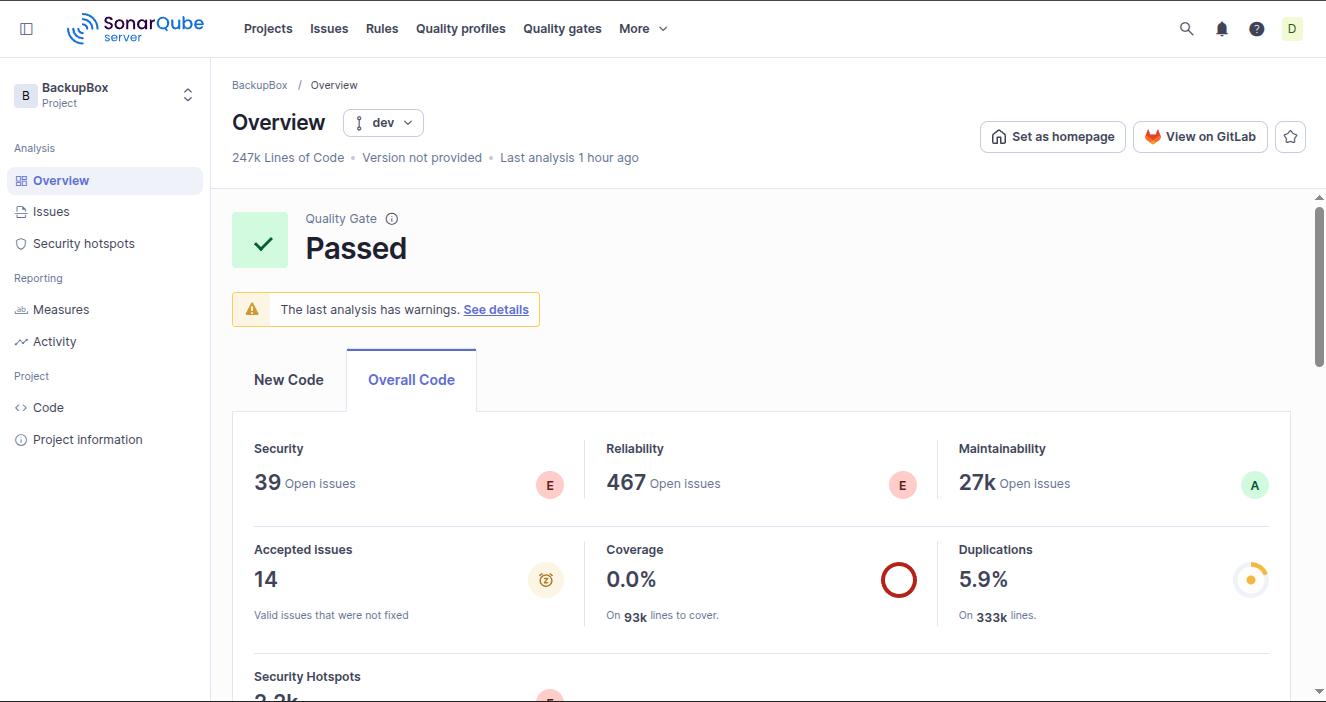
\includegraphics[width=\textwidth]{assets/sonar-overview.png}\\[2pt]
      {\fontsize{8}{10}\selectfont\textcolor{muted}%
        {Tableau de bord SonarQube du firmware de la Beebox.}}
  \end{columns}
\end{frame}

% =====================================================================
%  Les symptômes, un par un
% =====================================================================
\begin{frame}{Les symptômes, un par un}
  % --- moitié gauche de la capture, zoomée, sur la moitié droite de l'écran ---
  \begin{tikzpicture}[remember picture,overlay]
    % on découpe l'affichage sur la seule moitié droite de la diapositive
    \clip (current page.north) rectangle (current page.south east);
    % image affichée à 2x : ancrée par sa gauche au centre, sa moitié gauche
    % remplit alors la moitié droite de l'écran (le reste est rogné par le clip)
    \node[anchor=west,inner sep=0pt] at (current page.center)
      {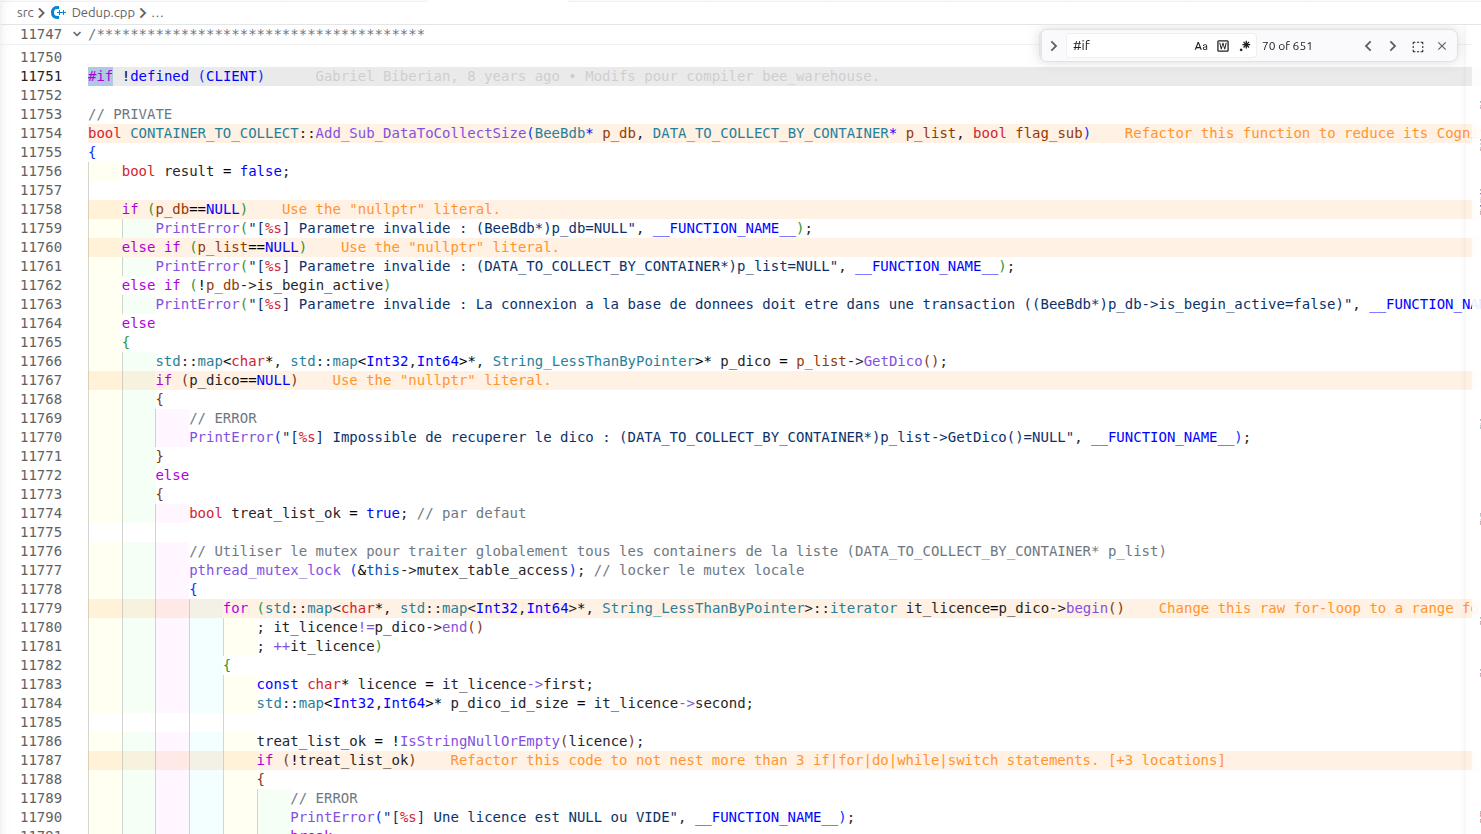
\includegraphics[width=\paperwidth]{assets/dedup-light.png}};
  \end{tikzpicture}
  \begin{columns}[c,onlytextwidth]
    \column{0.46\textwidth}
      \begin{itemize}\setlength\itemsep{0.34cm}
        \item Un \textbf{abus de directives de préprocesseur}
              (\texttt{\#ifdef}) pour gérer les cas de compilation.
        \item Des \textbf{fonctions interminables} et une maîtrise
              approximative du C++ (jusqu'à des tests
              \texttt{this == nullptr}, un \emph{undefined behavior}).
        \item Une \textbf{absence totale de tests} : aucun filet de sécurité.
        \item Un \texttt{main.h} qui \textbf{inclut tout le projet} : un
              couplage massif.
      \end{itemize}
    \column{0.50\textwidth}\mbox{}
  \end{columns}
\end{frame}

% =====================================================================
%  Le pattern : isoler le neuf du legacy (PIMPL)
% =====================================================================
\begin{frame}{Le pattern : isoler le neuf du legacy}
  \begin{columns}[c,onlytextwidth]
    \column{0.40\textwidth}
      \begin{itemize}\setlength\itemsep{0.30cm}
        \item Une \textbf{couche d'adaptation} (idiome \textbf{PIMPL}) joue le
              rôle de \textbf{frontière}.
        \item Tout le couplage avec le legacy est \textbf{confiné à une seule
              unité de traduction}.
        \item Le code neuf compile contre une \textbf{interface propre},
              \textbf{testable} et \textbf{isolée}.
      \end{itemize}
    \column{0.56\textwidth}
      \centering
      \resizebox{\textwidth}{!}{%
      \begin{tikzpicture}[font=\sffamily,
          legbox/.style={draw=muted,line width=1.2pt,fill=panel,rounded corners=6pt,
                         minimum height=1.9cm,text width=4.6cm,align=center,inner sep=8pt,text=ink2},
          newbox/.style={draw=accent,line width=1.3pt,fill=white,rounded corners=6pt,
                         minimum height=1.9cm,text width=4.6cm,align=center,inner sep=8pt,text=ink},
          wrapbox/.style={fill=accent,rounded corners=6pt,
                          minimum height=1.9cm,text width=4.6cm,align=center,inner sep=8pt,text=bg},
          biarr/.style={{Stealth[length=4mm,width=4mm]}-{Stealth[length=4mm,width=4mm]},
                        accent,line width=1.8pt}]
        \node[legbox]  (leg)  {\flowtxt{Legacy}{firmware historique, \texttt{main.h} qui inclut tout}};
        \node[wrapbox,right=1.5cm of leg] (wrap)
          {\flowtxthi{Couche d'adaptation}{idiome \textbf{PIMPL}, frontière unique}};
        \node[newbox,right=1.5cm of wrap] (new)
          {\flowtxt{Code neuf}{interface propre, testable, isolée}};
        \draw[biarr] (leg) -- (wrap);
        \draw[biarr] (wrap) -- (new);
      \end{tikzpicture}}
      \par\vspace{0.55cm}
      {\fontsize{10}{13}\selectfont\textcolor{muted}%
        {Le couplage reste confiné dans le \emph{wrapper} ; le neuf n'en dépend jamais directement.}}
  \end{columns}
\end{frame}

% =====================================================================
%  Automatiser un maximum de tâches
% =====================================================================
\begin{frame}{Automatiser un maximum de tâches}
  \vspace{0.45cm}
  \begin{columns}[t,onlytextwidth]
    \column{0.315\textwidth}
      \card{4.0cm}{Tester avant le \emph{merge}}{Le framework s'exécute en CI :
        un défaut est intercepté avant d'atteindre la production.}
    \column{0.315\textwidth}
      \cardhi{4.0cm}{Mesurer l'invisible}{Le bénéfice se compte en incidents
        qui n'ont jamais eu lieu, pas en incidents corrigés.}
    \column{0.315\textwidth}
      \card{4.0cm}{Industrialiser le reste}{Versionner les builds et rendre
        la compilation reproductible.}
  \end{columns}
\end{frame}

% =====================================================================
%  Construire proprement à côté : l'immuabilité
% =====================================================================
\begin{frame}{Construire proprement à côté : l'immuabilité}
  \vspace{0.30cm}
  \begin{columns}[t,onlytextwidth]
    \column{0.485\textwidth}
      \card{2.5cm}{La fonctionnalité}{Rendre un jeu de sauvegarde
        \textbf{insupprimable et inaltérable} pendant un délai de rétention.}
    \column{0.485\textwidth}
      \card{2.5cm}{Deux briques propres}{En \textbf{C++ moderne}, isolées et
        testables : un automate à états et un service de chiffrement.}
  \end{columns}
  \vspace{0.30cm}
  \begin{columns}[t,onlytextwidth]
    \column{0.485\textwidth}
      \card{2.5cm}{Sans aggraver la dette}{Écrite à côté du firmware qui
        l'accueille, jamais en l'alourdissant.}
    \column{0.485\textwidth}
      \cardhi{2.5cm}{L'enjeu métier}{Elle ferme un dernier angle d'attaque : la
        compromission de la box elle-même.}
  \end{columns}
\end{frame}

% =====================================================================
%  Conclusion
% =====================================================================
\begin{frame}{Conclusion}
  \vspace{0.30cm}
  \begin{columns}[t,onlytextwidth]
    \column{0.485\textwidth}
      \card{2.5cm}{Un arbitrage économique}{La dette est permanente, pas
        seulement un problème de code.}
    \column{0.485\textwidth}
      \card{2.5cm}{Une stratégie incrémentale}{Livrer tout en réduisant le
        risque des interventions suivantes.}
  \end{columns}
  \vspace{0.30cm}
  \begin{columns}[t,onlytextwidth]
    \column{0.485\textwidth}
      \cardhi{2.5cm}{La dette de connaissance}{La forme la plus dangereuse :
        elle part avec les personnes.}
    \column{0.485\textwidth}
      \card{2.5cm}{L'IA, un levier}{Elle récompense la compétence, sans jamais
        s'y substituer.}
  \end{columns}
\end{frame}

% =====================================================================
%  Ce que cette alternance m'a appris
% =====================================================================
\begin{frame}{Ce que cette alternance m'a appris}
  \vspace{0.45cm}
  \begin{columns}[t,onlytextwidth]
    \column{0.315\textwidth}
      \card{4.0cm}{Un spectre technique large}{C++ critique et embarqué, Python
        (un framework de 30 000 lignes), TypeScript, protocoles LSP/DAP,
        rétro-ingénierie.}
    \column{0.315\textwidth}
      \card{4.0cm}{Une compétence transversale}{Reprendre méthodiquement le
        contrôle d'un système opaque et non documenté.}
    \column{0.315\textwidth}
      \cardhi{4.0cm}{Deux contextes}{Un grand opérateur et une PME, et
        l'exercice exigeant de \textbf{transmettre}.}
  \end{columns}
\end{frame}

% =====================================================================
%  11 — REMERCIEMENTS / FIN
% =====================================================================
\begingroup
\setbeamercolor{background canvas}{bg=accent}
\begin{frame}[plain,c]
  \noindent
  {\seriffont\bfseries\fontsize{34}{38}\selectfont\textcolor{bg}{Merci de votre attention}\par}
  \vspace{0.35cm}
  {\fontsize{13}{17}\selectfont\textcolor{bg!85}%
    {Je remercie le jury et mes encadrants pour leur accompagnement,\\ et reste à votre disposition pour vos questions.}\par}
  \vspace{0.9cm}
  \begin{columns}[t]
    \column{0.40\textwidth}
      {\bfseries\fontsize{8}{10}\selectfont\textcolor{accentlt}{\MakeUppercase{Contact}}\par}
      \vspace{3pt}{\fontsize{11}{13}\selectfont\textcolor{bg}{jeremyhurel34@gmail.com}}
    \column{0.45\textwidth}
      {\bfseries\fontsize{8}{10}\selectfont\textcolor{accentlt}{\MakeUppercase{Structure d'accueil}}\par}
      \vspace{3pt}{\fontsize{11}{13}\selectfont\textcolor{bg}{Free Mobile · Beemo Technologie}}
  \end{columns}
  \vspace{0.9cm}
  % --- bandeau partenaires (cartouches blancs sur fond corail) ---
  \hbox{{\setlength{\fboxsep}{5pt}%
    \logochip{logo-um.png}{0.84cm}{0.92cm}\hspace{6pt}%
    \logochip{logo-free.png}{0.76cm}{0.92cm}\hspace{6pt}%
    \logochip{logo-beemo.png}{0.58cm}{0.92cm}}}
\end{frame}
\endgroup


\end{document}
